\documentclass[12pt,a4paper]{article}
\usepackage[utf8]{inputenc}
\usepackage{amsmath, amssymb, amsfonts}
\usepackage{geometry}
\geometry{margin=2.5cm}
\usepackage{hyperref}
\usepackage{pgfplots}
\usepackage{fancyhdr}
\usepackage{titlesec}
\titleformat{\section}
  {\normalfont\Large\bfseries\centering}  % Format: font size, bold, centered
  {\thesection}{1em}{} 
\pagestyle{fancy}
\pgfplotsset{compat=1.18}
\fancyhead{}
\fancyfoot{}
\title{Analisi Matematica 1}
\author{}
\date{}
\fancyhead[L]{Gabriele Perna}          % Left side
\fancyhead[C]{Analisi 1}     % Center
\fancyhead[R]{2025/2026}             % Right side
\fancyfoot[C]{\thepage}           % Page number in the center of footer
\let\oldsection\section
\renewcommand{\section}{\clearpage\oldsection}

\begin{document}

\maketitle
\tableofcontents
\section{Dizionario}

\begin{align*}
\subseteq &\quad \text{sottoinsieme} \\
\subset &\quad \text{sottoinsieme ma NON uguale a} \\
\exists &\quad \text{esiste} \\
\not\exists &\quad \text{NON esiste} \\
\cap &\quad \text{intersezione} \\
\cup &\quad \text{unione} \\
> &\quad \text{strettamente maggiore di} \\
< &\quad \text{strettamente minore di} \\
\ge &\quad \text{debolmente maggiore di} \\
\le &\quad \text{debolmente minore di} \\
\forall &\quad \text{per ogni}
\end{align*}

\section{Insiemi numerici}

\begin{itemize}
\item $\mathbb{N} \to$ Numeri naturali (interi non negativi)  
$\{0,1,2,3,4,5,\dots\}$
\item $\mathbb{Z} \to$ Numeri interi (interi positivi e negativi)  
$\{\dots,-3,-2,-1,0,1,2,3,\dots\}$
\item $\mathbb{Q} \to$ Numeri razionali  
Include le frazioni di forma $P/Q$ dove $P,Q \in \mathbb{Z}$, $Q \neq 0$  
Due frazioni diverse possono rappresentare lo stesso numero (½ e ¼)
\item $\mathbb{R} \to$ Numeri reali, contiene i precedenti e include molto di più ($\pi, e, \sqrt{2}, \dots$)
\end{itemize}

Si può dire che:  
\[
\mathbb{N} \subset \mathbb{Z} \subset \mathbb{Q} \subset \mathbb{R}
\]

\section{Intervalli}

Un insieme: $I \subset \mathbb{R}$  

Può essere definito intervallo se:  
\[
\forall x,y \in I, x<y \implies \forall z, x<z<y \Rightarrow z \in I
\]

ESEMPIO: $\mathbb{R} \setminus \{0\}$ NON è un intervallo.

\subsection{Intervalli di $\mathbb{R}$}

\begin{align*}
\text{Intervallo chiuso} &= [a,b] \\
\text{Intervallo aperto} &= (a,b) \\
\text{Intervallo semi-aperto / semi-chiuso} &= [a,b) \\
\text{Semiretta chiusa} &= [a,+\infty) \\
\text{Semiretta aperta} &= (a,+\infty) \\
\mathbb{R} &= (-\infty,+\infty)
\end{align*}

\section{Funzioni}

Una funzione consiste in una terna di oggetti: $f(A)=B$  

\begin{itemize}
\item $f$ = regola che assegna ad ogni elemento di $A$ uno e uno solo degli elementi di $B$.
\item $A$ = dominio
\item $B$ = codominio
\end{itemize}

Se dominio e codominio non vengono specificati, è sottointeso che:  
\[
A \subseteq \mathbb{R} \text{ più grande possibile in cui } f \text{ ha senso ed esiste, e } B = \mathbb{R}.
\]

\subsection{Grafico della funzione}

Il grafico di una funzione rappresenta un sottoinsieme di tutte le coppie $(a,b)$ con:  
\[
a \in A \quad \&\& \quad b \in B
\]

\subsection{Funzione iniettiva}

\[
\forall x_1,x_2 \in A, x_1 \neq x_2 \implies f(x_1) \neq f(x_2)
\]

\subsection{Funzione suriettiva}

\[
\forall y \in B, \exists x \in A : f(x)=y
\]

\subsection{Funzione biunivoca}

Funzione biunivoca, bigiettiva o invertibile se è suriettiva e iniettiva.  
Una funzione del genere può essere invertita, facendo la simmetria rispetto al grafico della funzione $f(x)=y$.  
\begin{align*}
    &f(x)=x^2\\
    &f(x^2)= x\\
    &f(x) = \sqrt{x}
\end{align*} 

\subsection{Funzione monotona}

Se abbiamo:  
$f(A)=B \quad \&\& \quad x_1,x_2 \in A \quad \&\& \quad x_1<x_2$  

Se $\forall x_1,x_2$ si calcolano le immagini e:  
\begin{align*}
f(x_1)<f(x_2) &\Rightarrow \text{funzione strettamente crescente} \\
f(x_1)>f(x_2) &\Rightarrow \text{funzione strettamente decrescente} \\
f(x_1)\le f(x_2) &\Rightarrow \text{funzione debolmente crescente} \\
f(x_1)\ge f(x_2) &\Rightarrow \text{funzione debolmente decrescente} \\
f(x_1)=f(x_2) &\Rightarrow \text{funzione costante}
\end{align*}

\textbf{OSSERVAZIONE:} Le funzioni strettamente monotone sono sempre iniettive.  

\subsection{Composizione di funzioni monotone}

Siano $A,B,C \in \mathbb{R}$, $f(A)=B$, $g(B)=C$:  
\[
g \circ f \to g(f(A)) = C
\]

\begin{itemize}
\item Se le due funzioni sono crescenti, la funzione composta è crescente
\item Se le due funzioni sono decrescenti, la funzione composta è crescente
\item Se una delle due funzioni è decrescente, la funzione composta è decrescente
\end{itemize}

\subsection{Funzioni pari e dispari}

\[
\text{Funzione pari: } f(x)=f(-x), \quad \text{Funzione dispari: } f(x)=-f(-x)
\]

\section{Funzioni elementari}

\subsection{Funzioni lineari}
$f(x)=ax+b, \quad a,b \in \mathbb{R}$\\\\
Esempio: $y=2x$  \\
$a = $ coefficiente angolare, $b = $ intercetta\\
Tutte le funzioni lineari sono suriettive e iniettive a meno che $a=0$

\subsection{Funzione potenza}
$y=x^n, n\in \mathbb{N}$  \\\\
Dominio: $\mathbb{R}$ \\ 
Esempio: $y=x^2$

\subsection{Funzione esponenziale}
$y=a^x$ \\\\ 
Esempio: $y=e^x$  \\
Inversa: $y=\log_a x$

\subsection{Funzione trigonometrica}
$y=\sin x$, \\$y=\cos x$, \\$y=\tan x$\\\\  
Funzioni inverse limitate a $[-\pi/2,\pi/2]$, codominio $[-1,1]$  

\subsection{Funzione periodica}
???

\section{Operazioni sui grafici}
\begin{align*}
\text{Traslazione verso l'alto: } & g(x)=f(x)+a, a>0 \\
\text{Traslazione verso il basso: } & g(x)=f(x)+a, a<0 \\
\text{Traslazione verso sinistra: } & g(x)=f(x+a), a>0 \\
\text{Traslazione verso destra: } & g(x)=f(x+a), a<0 \\
\text{Valore assoluto: } & g(x)=|f(x)| \\
\text{Simmetria rispetto asse X: } & g(x)=-f(x) \\
\text{Doppia simmetria o rotazione di 180°: } & g(x)=-f(-x)
\end{align*}

\section{Massimo, minimo ed estremi di insiemi}
\subsection{Massimo e minimo}
Il massimo di un insieme A è l'elemento che è maggiore o uguale a tutti gli elementi di A (incluso se stesso). 
\begin{align*}
M&=\max(A), M \in A \\
M(A) &= \{ M \in \mathbb{R} : a \le M, \forall a \in A \}
\end{align*}
La definizione è analoga per il minimo di un insieme.

\subsection{Maggiorante e minorante}
Un maggiorante di un insieme A è un elemento che è maggiore di tutti gli elementi di A non sempre però appartenente ad A.
L'insieme dei maggioranti di A si definisce cosi:
\begin{align*}
    M_A = \{\forall a \in A, a \le M\}
\end{align*}
L'insieme dei maggioranti di $\mathbb{R}$ è $\emptyset$\\
La definizione è analoga per i minoranti di un insieme.

\subsection{Insiemi limitati}
Un insieme A è superiormente limitato se ha un estremo superiore, ovvero:
\begin{align*}
    M_A \ne \emptyset
\end{align*}
La definizione è analoga per un insieme inferiormente limitato.\\
Un insieme è limitato se è superiormente e inferiormente limitato.

\subsection{Estremi}
Se un insieme A è superiormente limitato allora esiste l'insieme $M_A$.\\
L'elemento minore di $M_A$ viene detto \textbf{estremo superiore} di A.\\
Se A non è superiormente limitato allora l'estremo superiore di A è $+\infty$.
\paragraph{OSSERVAZIONE:} Se l'estremo superiore di A $\in$ A allora A ha un massimo.\\
La definizione è analoga per l'\textbf{estremo inferiore}.

\section{Operazioni vietate}
\[
\infty + (-\infty), \quad 0 \cdot (\pm \infty)
\]

\section{Parte intera}
\[
[x] = \max \{ m \in \mathbb{Z} : m \le x \}
\]

\section{Massimo, minimo ed estremi di funzioni}

\subsection{Massimo e minimo}
Una funzione $f(A) \rightarrow \mathbb{R}$ ha massimo se $f(a)$ ha massimo.\\
La definizione è analoga per il minimo di una funzione.

\subsection{Estremi di una funzione}
L'estremo superiore di una funzione corrisponde all'estremo superiore dell'immagine.\\
La definizione è analoga per l'estremo inferiore.

\subsection{Punti di massimo}
I punti di massimo di una funzione sono i valori delle X per cui si ottiene il valore massimo dell'immagine.

\subsection{Affermazioni importanti}
A patto che la funzione abbia minimo e massimo:
\begin{align*}
\text{Se f è debolmente crescente: } & \max(f)=f(\max(A)), \quad \min(f)=f(\min(A)) \\
\text{Se f è debolmente decrescente: } & \max(f)=f(\min(A)), \quad \min(f)=f(\max(A))
\end{align*}

\section{Continuità di una funzione}
$f(A)\to \mathbb{R}$ è continua in $x_0$ se:
\[
\forall \epsilon >0 \ \exists \delta >0 : x\in A, |x-x_0|<\delta \Rightarrow |f(x)-f(x_0)|<\epsilon\\
\]
Inoltre, la funzione deve essere continua nel suo dominio, non bisogna farsi inganare dai falsi vuoti.\\
Solo i salti nell'immagine rendono una funzione non continua.

\subsection{Continuità nelle funzioni elementari}
\begin{align*}
    \text{Funzione costante: } y &= k , \text{continua.}\\
    \text{Funzione lineare: } y &= x , \text{continua.}\\
    \text{Polinomio: } &P(x) , \text{continua.}\\
    \text{Funzione razionale: } &\frac{P(x)}{P(q)} , \text{continua.}\\
    \text{Funzione trigonometrica: } sin(x)&,cos(x)\ldots \text{continua.}\\
    \text{Funzione esponenziale: } &e^x , \text{continua.} 
\end{align*}
Per quanto riguarda la composizione di funzioni:\\
Se due funzioni continue vengono composte allora la funzione risultante sarà continua.

\subsection{Teorema di esistenza degli zeri}
Se $f:[a,b] \rightarrow \mathbb{R}$ è continua e $f(a) * f(b) < 0$ allora:
\[
\exists c \in (a,b) : f(c) = 0
\]
\subsection{Teorema dei valori intermedi}
Se una funzione $f:I \rightarrow \mathbb{R}$ con $I = [a,b]$ si può dire che $f(I)$ è un intervallo.

\subsection{Teorema di Weierstrass}
Se una funzione $f:[a,b] \rightarrow \mathbb{R}$ è continua ammette minimo e massimo.

\section{Intorni}
Un intorno di $x_0$ si può definire così:
\[
\{x_0 - \epsilon, x_0 + \epsilon\}, \epsilon > 0, \epsilon \in \mathbb{R}
\]
Se $x_0 = +\infty$ il suo intorno è una semiretta $(a,+\infty), a \in \mathbb{R}$.
Per $x_0 = -\infty$ l'intorno invece è la semiretta $(-\infty, a), a \in \mathbb{R}$.

\subsection{Punti di accumulazione}
$x_0$ è definito \textbf{punto di accumulazione} dell'insieme A se:
\begin{align*}
    (U \cap A) \setminus \{x_0\} \ne \emptyset \\ 
    U = \text{intorno di } x_0
\end{align*}
L'insieme dei punti di accumulazione di A si indica con $acc(A)$.\\
I punti che non fanno parte di $acc(A)$ sono \textbf{punti isolati}.

\subsection{Punti di massimo e minimo locale}
$x_0$ è definito \textbf{punto di massimo locale} se:
\[
\forall x \in U \cap A : f(x) \le f(x_0)
\]
La definizione è analoga per i \textbf{punti di minimo locale}.\\\\
$x_0$ è definito \textbf{punto di massimo locale stretto} se:
\[
\forall x \in U \cap A : f(x) < f(x_0)
\]
La definizione è analoga per i \textbf{punti di minimo locale stretto}.

\section{Limiti}
Un \textbf{limite} indica il valore a cui l'immagine di una funzione si avvicina all'avvicinarsi di $x$ a $x_0$.
\[
\lim_{x \to x_0} f(x)  
\]
'Limite per x che tende a $x_0$ di $f(x)$'\\\\
Il \textbf{teorema di unicità al limite} dice che se un limite esiste allora è unico.\\
Intuitivamente, un limite può non esistere.

\subsection{Teoremi, definizioni e proprietà}
\begin{itemize}
  \item La somma o il prodotto di due limiti vale se ha senso (no operazioni vietate).
  \item Se esiste $\lim_{x \to x_0} f(x) = l$ con $l \in R$ ('Esiste finito il limite') allora vicino a $x_0$ la funzione è limitata. 
  \item Se $\lim_{x \to x_0} f(x) = 0$ si dice che $f(x)$ è \textbf{infinitesima} per $x \rightarrow x_0$
  \item Se una funzione è strettamente crescente allora:
  \begin{itemize}
    \item $\lim_{x \to a^+} f(x) = inf(f(x))$
    \item $\lim_{x \to b^-} f(x) = sup(f(x))$
  \end{itemize}
  \item Se $\lim_{x \to x_0} f(x) = 0^+$ allora$\lim{x \to x_0} \frac{1}{f(x)} = +\infty$, analogo per:
  \begin{itemize}
    \item $0^- \rightarrow -\infty$
    \item $+\infty \rightarrow 0^+$
    \item $-\infty \rightarrow 0^-$
    \item $l \in \mathbb{R} \rightarrow \frac{1}{l}$
  \end{itemize}
\end{itemize}

\subsection{Limiti fondamentali}

\begin{align*}
&\lim_{x \to +\infty} x = +\infty\\
&\lim_{x \to +\infty} x^n = +\infty * (+\infty) * (+\infty)\cdots = +\infty\\
&\lim_{x \to +\infty} \frac{1}{x} = 0^+\\
&\lim_{x \to +\infty} P(X) = +\infty \text{se il monomio dominante} > 0, -\infty \text{ se} <0\\
&\lim_{x \to +\infty} e^x = +\infty\\
&\lim_{x \to -\infty} e^x = 0\\
&\lim_{x \to +\infty} log(x) = +\infty\\
&\lim_{x \to 0^+} log(x) = -\infty
\end{align*}

\subsection{Teorema dei carabinieri}

Il \textbf{Teorema dei Carabinieri} (o \emph{teorema del confronto}) afferma che se tre funzioni $f(x)$, $g(x)$ e $h(x)$ sono tali che:

\[
f(x) \leq g(x) \leq h(x) \quad \text{per ogni } x \text{ in un intorno di } x_0,
\]
e se
\[
\lim_{x \to x_0} f(x) = \lim_{x \to x_0} h(x) = L,
\]
allora
\[
\lim_{x \to x_0} g(x) = L.
\]

Questo teorema è molto utile quando si vuole calcolare il limite di una funzione complessa $g(x)$, ma si riescono a trovare due funzioni più semplici che la ``schiacciano'' e che tendono allo stesso limite.

\vspace{1em}

\textbf{Esempio:} Calcoliamo
\[
\lim_{x \to 0} x^2 \sin\left(\frac{1}{x}\right).
\]
Poiché $-1 \leq \sin\left(\frac{1}{x}\right) \leq 1$, moltiplicando per $x^2$ (che è sempre positivo vicino a $0$), otteniamo:
\[
- x^2 \leq x^2 \sin\left(\frac{1}{x}\right) \leq x^2.
\]
Poiché $\lim_{x \to 0} (-x^2) = \lim_{x \to 0} (x^2) = 0$, per il Teorema dei Carabinieri si ha:
\[
\lim_{x \to 0} x^2 \sin\left(\frac{1}{x}\right) = 0.
\]

\vspace{1em}

\textbf{Visualizzazione:}

\begin{center}
\begin{tikzpicture}[scale=5]
  \draw[->] (-0.6,0) -- (0.6,0) node[right] {$x$};
  \draw[->] (0,-0.6) -- (0,0.6) node[above] {$y$};

  \draw[domain=-0.5:0.5,smooth,variable=\x,blue,thick] 
    plot ({\x},{\x*\x}) node[right] {$y = x^2$};
  \draw[domain=-0.5:0.5,smooth,variable=\x,red,thick] 
    plot ({\x},{-\x*\x}) node[right] {$y = -x^2$};
  \draw[domain=-0.5:0.5,smooth,variable=\x,orange,thick] 
    plot ({\x},{(\x*\x)*sin(1/(\x))}) node[below right] {$y = x^2 \sin\left(\tfrac{1}{x}\right)$};

  \node at (0.05,0.05) {$0$};
\end{tikzpicture}
\end{center}

Come si vede nel grafico, la funzione $x^2 \sin\left(\tfrac{1}{x}\right)$ è sempre compresa tra $-x^2$ e $x^2$, e ``si schiaccia'' verso $0$ con esse.

\vspace{1em}

Questo teorema prende il nome di "teorema dei carabinieri" poiché, come due carabinieri che accompagnano un sospetto verso una destinazione, le due funzioni $f(x)$ e $h(x)$ guidano la funzione $g(x)$ verso il loro stesso limite.

\subsection{Teorema di Weierstrass generalizzato}

Se:
\begin{itemize}
    \item Una funzione $f(a,b) \rightarrow \mathbb{R}$ è continua.
    \item Il limite $l_1 = \lim_{x \to a^+}$ esiste.
    \item Il limite $l_2 = \lim_{x \to b^-}$ esiste.
\end{itemize}
Allora si può dire che
\begin{itemize}
    \item $f$ è limitata inferiormente $\Leftrightarrow$ $l_1 \ne -\infty$ e $l_2 \ne -\infty$
    \item $f$ è superiormente limitata $\leftrightarrow$ $l_1 \ne +\infty$ e $l_2 \ne +\infty$
    \item $f$ ha minimo $\leftrightarrow$ $\exists x_0 \in (a,b) : f(x_0) \le min \{l_1,l_2\}$
    \item $f$ ha massimo $\leftrightarrow$ $\exists x_0 \in (a,b) : f(x_0) \ge max \{l_1,l_2\}$
    \item $f$ è limitata $\leftrightarrow$ $l_1,l_2 \in \mathbb{R}$
\end{itemize}

\section{Infinitesimi}
\subsection{O piccolo}
Si dice che $f(x)$ è \textbf{o-piccolo} di g(x) per $x$ che tende a $x_0$ e si scrive cosi:
\[
f(x) = o(g(x)) \text{ per } x \rightarrow x_0
\]
Se:
\[
\lim_{x \to x_0} \frac{f(x)}{g(x)} = 0
\]
Ovvero quando $f(x)$ cresce più lentamente.
Si dice anche che $f(x)$ è \textbf{trascurabile} rispetto a $g(x)$\\
\subsection{Omega piccolo}
L'opposto di o-piccolo è \textbf{omega-piccolo}, che si può indicare come $\omega(x)$.
\[
f(x) = \omega(g(x))
\]
Se:
\[
\lim_{x \to x_0} \frac{f(x)}{g(x)} = +\infty
\]
Da queste definizioni iniziali possiamo trarre che:
\[
f(x) = o(g(x)) \Longleftrightarrow f(x) = g(x) \cdot \omega(x) \Longleftrightarrow g(x) = \omega(f(x))
\]
Ciò significa che la condizione di o-piccolo è vera se esiste un omega-piccolo in grado di provare la condizione opposta.
\subsection{O grande}
Non si usa più spesso, ma \textbf{O grande} ma:
\[
f(x) = O(g(x))
\]
Significa che $f(x)$ cresce al massimo come g, a meno di una costante moltiplicativa, per $n$ abbastanza grande.
\[
f(n) = O(g(n))
\quad \Longleftrightarrow \quad
\exists\, c > 0,\, n_0 \in \mathbb{R}^+ \text{ tali che } 
\forall n > n_0,\; 0 \le f(n) \le c\, g(n)
\]

\section{Asintoti}

Per una funzione ci possono essere al più un asintoto orizzontale o obliquo per $x \rightarrow +\infty$
e al più uno per $x \rightarrow -\infty$.
Ci possono invece essere infiniti asintoti verticali.

\subsection{Asintoto orizzontale}
Se abbiamo una funzione $f:(a,+\infty) \rightarrow \mathbb{R}$ con $a \in \overline{\mathbb{R}}$ ed esiste il limite
$\lim_{x \to +\infty} f(x) = l \in \mathbb{R}$ (non $+ o - \infty$), allora si dice che $f(x)$ ha la retta orizzontale $y=l$ come \textbf{asintoto orizzontale} per $x \rightarrow +\infty$

\subsection{Asintoto verticale}
Se il limite per $x_0$ è $+ o - \infty$ da almeno una parte, allora $x = x_0$ è un \textbf{asintoto verticale} della funzione.

\subsection{Asintoto obliquo}
Se abbiamo una funzione $f:(a,+\infty) \rightarrow \mathbb{R}$ con $a \in \overline{\mathbb{R}}$ e se esiste il limite:\\
\[\lim_{x \to +\infty} \frac{f(x)}{x} = m, m \ne 0\]
ed esiste:\\
\[\lim_{x \to +\infty} f(x) - mx = q \in \mathbb{R}\]
Allora $y = mx + q$ è l'\textbf{asintoto obliquo} della funzione per $x \rightarrow + \infty$

\section{Derivate}
\subsection{Definizione}
Se esiste il limite:
\[
\lim_{x \to x_0} \frac{f(x) - f(x_0)}{x-x_0} = \lim_{x \to {x_0}^+} \frac{\Delta f}{\Delta x} = l 
\]
Si dice che $l$ è la \textbf{derivata} di $f$ in $x_0$, con $l \in \overline{\mathbb{R}}$\\\\
$f$ si dice \textbf{derivabile} in $x_0$ se:
\[
\exists l, l \in \mathbb{R}
\]
La derivata di una funzione si indica in questo modo:
\begin{itemize}
  \item $f^|(x_0)$
  \item $Df(x_0)$
\end{itemize}
Graficamente, tramite il calcolo della derivata si trova la pendenza (coefficiente angolare) della retta secante al grafico di $f$
che passa per i punti $(x_0,f(x_0)),(x,f(x))$.
\begin{center}
  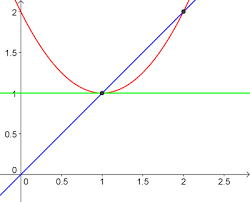
\includegraphics[width=0.5\textwidth]{images/rettasecantederivata.png}
\end{center}
Quando $x \rightarrow x_0$ la retta secante tende alla retta tangente al grafico di $x_0$.
\begin{center}
  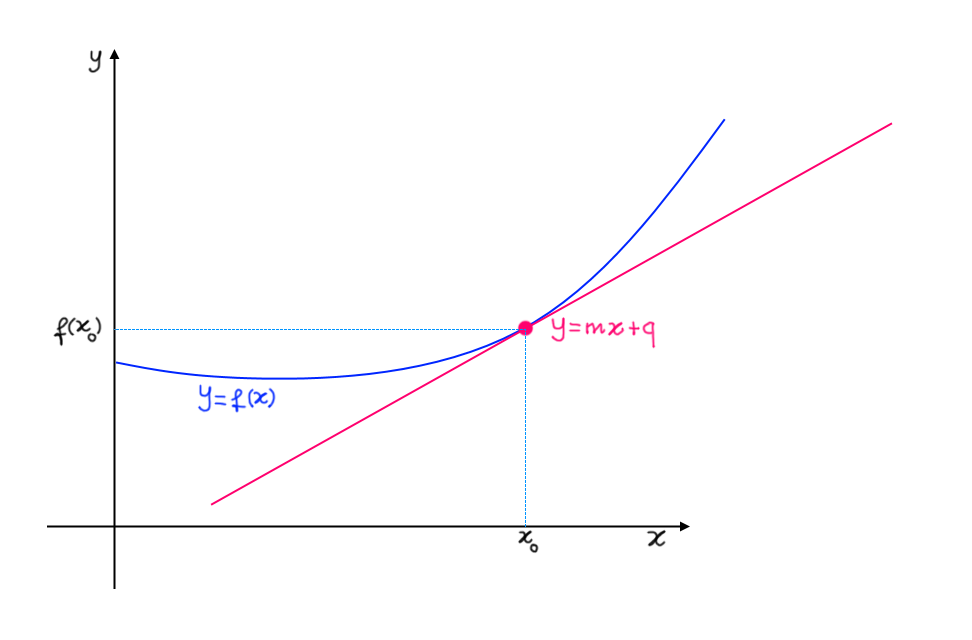
\includegraphics[width=0.5\textwidth]{images/rettatangentederivata.png}
\end{center}
Se una funzione è derivabile in $x_0$, allora è continua in $x_0$, ma il contrario non è sempre vero.\\

\subsection{Derivata destra e sinistra}
Se esiste il limite:
\[
\lim_{x \to {x_0}^+} \frac{f(x) - f(x_0)}{x-x_0} = \lim_{x \to {x_0}^+} \frac{\Delta f}{\Delta x} = l 
\]
Si dice che l è la \textbf{derivata destra} di $f$ in $x_0$.\\
La definizione è analoga per la \textbf{derivata sinistra}.\\
Una funzione è derivabile in un punto se la derivata destra e la derivata sinistra sono uguali e se sono finiti (non $\pm \infty$).
\paragraph{Punto angoloso: } punto in cui le derivate destra e sinistra esistono ma sono diverse.
\paragraph{Cuspide (o singolarità): } se la derivata destra e sinistra sono rispettivamente $+ \infty$ e $- \infty$ (o viceversa) allora si dice che $f$ ha una cuspide in $x_0$.\\
In questo caso la tangente delle derivate destra e sinistra è la stessa.

\subsection{Funzione derivata}
Se $f: A \rightarrow \mathbb{R}$ è derivabile $\forall x_0 \in A$ si definisce la \textbf{funzione derivata} $f^|(x)$ che associa ad ogni $x_0$ il suo $f^|(x_0)$.\\
La funzione derivata può a sua volta avere una sua funzione derivata.\\\\
Si dice che $f$ è di classe $C^n$ se è derivabile $n$ volte e $f^n$ è continua.

\subsection{Derivate notevoli ed equivalenze}
\begin{itemize}
  \item $D(k) = 0$
  \item $D(x) = 1$
  \item $D(x^2) = D(x \cdot x) = 2x$
  \item $D(x^n) = n \cdot x^{n-1}$
  \item $D(e^x) = e^x$
  \item $D(cosx) = -sinx$
  \item $D(sinx) = cosx$
  \item $D(tgx) = D(\frac{sinx}{cosx}) = \frac{1}{cos^2x} = 1 + tg^2x$
  \item $D(k \cdot f) = k \cdot D(f)$
  \item $D(logx) = \frac{1}{x}$
  \item $D(k^x) = k^x \cdot log(k)$
\end{itemize}
Se $f$ e $g$ sono derivabili in $x_0$ allora:
\begin{itemize}
  \item $(f+g)^|(x_0) = f^|(x_0) + g^|(x_0)$
  \item $(f\cdot g)^|(x_0) = f^|(x_0) \cdot g(x_0) + f(x_0) \cdot g^|(x_0)$
\end{itemize}
Se $f(x_0) \ne 0$ allora:
\begin{itemize}
  \item $(\frac{1}{f})^| (x_0) = \frac{f^|(x_0)}{f(x_0)^2} $
\end{itemize}
Se $f$ è derivabile in $x_0$ e $f(x_0) \ne 0$ allora la derivata della funzione inversa è:
\begin{itemize}
  \item $f^{-1}(y_0) = \frac{1}{f^|(x_0)} = \frac{1}{f^|(f^{-1}(y_0))}$
\end{itemize}
Se $f$ e $g$ sono derivabili nel loro dominio allora:
\begin{itemize}
  \item $(g o f)^| = g^|(f(x_0)) \cdot f^|(x)$
\end{itemize}

\subsection{Teorema di Fermat}
Data una funzione $f: A \rightarrow \mathbb{R}$, $x_0$ come punto interno ad $A$ (non sul bordo) che sia di massimo o minimo locale (o assoluto)
e $f$ derivabile in $x_0$ allora:
\[
f^|(x_0) = 0
\]
La retta tangente è perfettamente orizzontale, inizia a riscendere / risalire.

\subsection{Teorema di Rolle}
Data una funzione $f:[a,b] \rightarrow \mathbb{R}$ continua, se $[a,b]$ è derivabile in $(a,b)$ e se $f(a) = f(b)$ allora:
\[
\exists c \in (a,b) : f^|(c) = 0
\]
Ovvero esiste almeno un punto $c$ dove la derivata è 0.\\\\
Il teorema è facilmente dimostrabile:
\begin{itemize}
  \item La funzione è continua e secondo il teorema di Weierstrass ammette minimo e massimo.
  \item Secondo il teorema di Fermat, ogni punto di minimo e massimo ha come derivata 0.
\end{itemize}
\paragraph{Osservazione: } se $f(a) = min(f)$ e $f(b) = max(f)$ o viceversa la funzione è costante.

\subsection{Teorema di Lagrange ("Rolle storto")}
Data una funzione $f:[a,b] \rightarrow \mathbb{R}$ continua, derivabile in $(a,b)$ allora:
\[
\exists c \in (a,b) : f^|(c) = \frac{f(b) - f(a)}{b - a}
\]
Ovvero esiste almeno un punto la cui retta tangente della derivata è parallela alla retta della derivata dell'intera funzione.
\paragraph{Conseguenze del teorema di Lagrange:} data $f:I \rightarrow \mathbb{R}$ continua e derivabile nella parte interna di $I$ possiamo dire che:
\begin{itemize}
  \item Se $f^|(x) = 0$, $\forall x \in int(I) \rightarrow f$ è costante in $I$
  \item Se $f^|(x) \geq 0$, $\forall x \in int(I) \rightarrow f$ è debolmente crescente in $I$
  \item Se $f^|(x) \leq 0$, $\forall x \in int(I) \rightarrow f$ è debolmente decrescente in $I$
  \item Se $f^|(x) > 0$, $\forall x \in int(I) \rightarrow f$ è strettamente crescente in $I$
  \item Se $f^|(x) < 0$, $\forall x \in int(I) \rightarrow f$ è strettamente decrescente in $I$
\end{itemize}
\paragraph{Proprietà: } data $f:I \rightarrow \mathbb{R}, x0 \in I, f$ derivabile in $I \setminus {x_0}$ e continua su $I$, allora:
\begin{itemize}
  \item Se $f(x)^|\leq 0$ in un intorno sinistro di $x_0$ e $f(x)^| \geq 0$ in un intorno destro di $x_0$ allora $x_0$ è un punto di minimo locale per $f$.
  \item Se $f(x)^|\geq 0$ in un intorno sinistro di $x_0$ e $f(x)^| \leq 0$ in un intorno destro di $x_0$ allora $x_0$ è un punto di minimo locale per $f$.
\end{itemize}

\subsection{Derivata seconda}
Data $f:A \rightarrow \mathbb{R}, x_0 \in int(A)$, supponiamo che la funzione sia derivabile in $x_0$ due volte e che $f^|(x_0) = 0$:
\begin{itemize}
  \item Se $x_0$ è minimo locale allora $f^{||}(x_0) \geq 0$
  \item Se $x_0$ è massimo locale allora $f^{||}(x_0) \leq 0$
  \item Se $f^{||}(x_0) > 0$ allora $x_0$ è minimo locale
  \item Se $f^{||}(x_0) < 0$ allora $x_0$ è massimo locale
\end{itemize}

\subsection{Teorema di l'Hopital}
Dati $a,b \in \overline{\mathbb{R}}, f,g: (a,b) \rightarrow \mathbb{R}$ derivabili in $(a,b)$, se:
\begin{enumerate}
  \item $\lim_{x \to a^+} \frac{f(x)}{g(x)}$ è indeterminato
  \item $g^|(x) \ne 0$
  \item $\exists \lim_{x \to a^+} \frac{f^|}{g^|(x)} = l \in \overline{\mathbb{R}}$
\end{enumerate}
Allora:
\[
\exists \lim_{x \to a^+} \frac{f(x)}{g(x)} = l
\]
Analogo se applicato a $b^-$.

\subsection{Sviluppo di Taylor}
\subsection{Fattoriale}
\begin{align*}
  0! &= 1\\
  1! &= 1\\
  n! &= n \cdot (n-1)!\\
\end{align*}
\subsection{Sommatoria}
Se $aj \in \mathbb{R}$ indicizzati da numeri naturali.
\[
\sum_{j=m}^h aj \rightarrow am + \ldots + an
\]
\subsection{Formula di Taylor}
Se $f$ è derivabile in $x0 \in (a,b)$ abbiamo:
\[
f(x) = f(x_0) + f^|(x_0) \cdot (x-x_0) + o(x-x_0)
\]
La \textbf{Formula di Taylor} ci da un approssimzione più precisa (aumentando il grado del polinomio sopra riportato).\\
L'idea è che più è alto il grado, più è corretta l'approssimazione.
\paragraph{Formula di Taylor con formula di Peano: } se $f(a,b) \rightarrow \mathbb{R}$, $x_0 \in (a,b)$, $f$ derivabile $n-1$ volte in $(a,b)$ e $n$ volte in $x_0$ allora esiste un unico polinomio
di grado $n$ chiamato $Pn(x)$ tale che:
\[
f(x) = Pn(x) + o((x-x_0)^n) per x \to x_0
\]
$Pn(x)$ ha la seguente forma:
\[
Pn(x) = \sum_{j=0}^n \frac{f^j(x_0)}{j!} \cdot (x-x_0)^j
\]
\paragraph{Formula di Taylor con resto di Lagrange: } errore più controllabile.\\
Se $f(a,b) \rightarrow \mathbb{R}$, $x_0 \in (a,b)$, $f$ derivabile $n+1$ volte in $(a,b) \setminus {x_0}$ e $n$ volte in $x_0$ allora:
\[
f(x) = Pn(x) + Rn(x)
\]
dove:
\[
\forall (a,b) \exists zx \in (x_0,x) \lor \exists zx \in (x,x_0) : Rn(x) = \frac{f^{n+1}(zx)}{(n+1)!} \cdot (x-x_0)^{n+1}
\]
\section{Convessità}

\subsection{Funzione convessa}
Dato un intervallo $I \subset \mathbb{R}$ e una funzione $f : I \to \mathbb{R}$,  
$f$ si dice \emph{convessa} in $I$ se, presi due punti qualsiasi sul grafico, il segmento che li unisce è sopra il grafico di $f$.

In formule: per ogni $x_1, x_2 \in I$ con $x_1 < x_2$ e per ogni $t \in (0,1)$ vale
\[
f(x_1 + t(x_2 - x_1)) \le f(x_1) + t(f(x_2) - f(x_1)).
\]
Se la disuguaglianza è stretta ($<$), allora $f$ è \emph{strettamente convessa}.

\subsection{Funzione concava}
$f$ si dice concava se $-f$ è convessa.  
Strettamente concava se $-f$ lo è strettamente.\\
In formule:
\[
f(x_1 + t(x_2 - x_1)) \ge f(x_1) + t(f(x_2) - f(x_1)).
\]
Nota: se compare il simbolo $>$ invece di $\ge$, allora $f$ è strettamente concava.

\subsection{Calcolo della convessità}

Dato un intervallo $I \subset \mathbb{R}$ e una funzione $f : I \to \mathbb{R}$ derivabile due volte, sono equivalenti:

\begin{itemize}
  \item $f$ è convessa (risp. strettamente convessa);  
  \item $f'$ è debolmente crescente (risp. strettamente crescente);  
  \item $f'' \ge 0$ (risp. $f''>0$).
\end{itemize}
La stessa caratterizzazione vale per la concavità scambiando i segni.

\subsection{Interpretazione geometrica}

Dire che $f'$ è crescente significa che il coefficiente angolare della tangente cresce; la tangente, mentre ci si muove lungo il grafico, ``ruota in senso antiorario''.\\
Una funzione $f$ è convessa in $I$ se e solo se per ogni $x_0 \in I$ si ha:
\[
f(x) \ge f(x_0) + f'(x_0)(x - x_0),
\]
cioè il grafico sta sopra la retta tangente nel punto $(x_0, f(x_0))$.\\
Concava se vale il $\le$.  
Strettamente convessa se vale $>$ per $x \ne x_0$.  
Strettamente concava se vale $<$ per $x \ne x_0$.\\
La funzione $f(x_0) + f'(x_0)(x - x_0)$ rappresenta la retta tangente.\\
Sia $I \subset \mathbb{R}$ un intervallo, $x_0$ un punto interno e $f$ derivabile in $I \setminus \{x_0\}$.  
Siano $I_1 = \{x < x_0\}$ e $I_2 = \{x > x_0\}$.  
Se $f$ è convessa in $I_1$ e in $I_2$ e $x_0$ è angoloso, allora $f$ è convessa in tutto $I$ se e solo se:
\[
f'_-(x_0) \le f'_+(x_0).
\]

\subsection{Flessi}
Dato $I \subset \mathbb{R}$, una funzione $f : I \to \mathbb{R}$ e un punto interno $x_0$,  
$x_0$ è un \emph{punto di flesso} se $f$ è derivabile in $x_0$ ed esiste un intorno $U$ in cui
\[
\frac{f(x) - (f(x_0) + f'(x_0)(x - x_0))}{x - x_0}
\]
cambia segno.  
Ciò significa che il grafico passa da sopra a sotto la tangente, o viceversa.\\
\textbf{Flesso a tangente verticale: }  
se $f'(x_0)=\pm\infty$, $f$ è continua in $x_0$ e $f$ è convessa da un lato e concava dall'altro (o viceversa),  
allora $x_0$ è punto di flesso a tangente verticale.\\
Se $f$ è derivabile due volte e $f''(x_0)=0$ e cambia segno, allora $x_0$ è punto di flesso.  
Cambia segno significa:
\[
f''(x) \le 0 \text{ per } x<x_0, \qquad f''(x)\ge 0 \text{ per } x>x_0,
\]
oppure viceversa.\\
Il fatto che $f''(x_0)=0$ non è sufficiente per avere un flesso.  
Possono esistere flessi anche dove $f''$ non esiste.\\
Se una funzione $f : I \to \mathbb{R}$ è convessa nei punti interni di $I$ ed è continua in tutto $I$, allora è convessa in tutto $I$.  
In particolare: se $f$ è convessa in $(a,b)$ e continua in $[a,b]$, allora è convessa in $[a,b]$.

\section{Studio di funzione}

\subsection{Punti da seguire}

Dato $f(x)$, senza dominio esplicitato, si seguono questi passi:

\begin{itemize}
  \item determinare l’insieme di definizione;  
  \item determinare l’insieme di continuità;  
  \item determinare l’insieme di derivabilità;  
  \item studiare eventuali asintoti verticali, orizzontali o obliqui;  
  \item studiare la monotonia;  
  \item trovare eventuali massimi o minimi locali;  
  \item determinare massimo/minimo assoluto, oppure $\sup$ e $\inf$;  
  \item studiare la convessità e gli eventuali flessi.
\end{itemize}

\section{Integrali}
\subsection{Integrali di Riemann}
Data $d:[a,b] \rightarrow \mathbb{R}$ limitata, \textbf{l'integrale definito} di $f(x)$ su $[a,b]$ è un numero reale che rappresenta l'area del sottografico.\\
Una \textbf{suddivisione} di $[a,b]$ è un insieme di punti $x_0, x_1,\ldots, x_n$ con $a = x_0, x_1,\ldots, x_n = b$.\\
La lunghezza delle suddivisioni non è per forza la stessa. La somma delle lunghezze degli intervalli è uguale a $b-a$.\\
La \textbf{somma inferiore di $f$} relativa a una suddivisione $A$ è:
\[
S^|(f,A) = \sum_{i = 1}^{n} m_i \cdot (x_i - x_i - 1)
\]
Con:
\[
m = \text{valore della funzione minore del sottointervallo}
\]
La somma inferiore approssima l'area del grafico per difetto.\\
La definizione è analoga per la \textbf{somma superiore}, che considera $M$ come valore massimo e approssima l'area per eccesso.
\[
S^{||}(f,A) = \sum_{i = 1}^{n} M_i \cdot (x_i - x_i - 1)
\]
Se $S^| = S^{||}$ si dice che $f$ è integrabile su $[a,b]$ e il suo integrale definito è:
\[
\int_{a}^{b} f(x) dx = S^| = S^{||}
\]
Se $f \leq 0$, l'integrale corrisponde all'opposto dell'area del sottografico.\\
Se la funzione $f:[a,b]$ è continua o \textbf{generalmente continua}, allora è integrabile.\\
Una funzione è generalmente continua se è limitata e ha un numero finito di punti di discontinuità.\\\\
Se $f$ è integrabile, $S^{||} - S^|$ tende a $0$ al "raffinarsi delle suddivisioni".

\subsection{Proprietà}
Dati $f,g$ integrabili su $[a,b]$ e $k \in \mathbb{R}$:
\[
  f+g, k \cdot f, |f| \text{ sono integrabili}
\]
\begin{itemize}
  \item $\int_{a}^{b} (f(x) + g(x)) dx = \int_{a}^{b} f(x) dx + \int_{a}^{b} g(x) dx$
  \item $\int_{a}^{b} (k \cdot f(x)) dx = k \cdot \int_{a}^{b} f(x) dx$
  \item Se $f(x) \leq g(x)$ $\forall x \in (a,b)$ allora:
  \begin{itemize}
    \item $\int_{a}^{b} f(x) dx \leq \int_{a}^{b} g(x) dx$
  \end{itemize}
  \item $|\int_{a}^{b} f(x) dx| \leq \int_{a}^{b} |f(x)| dx$
  \item Se $a < c < b$ allora:
  \begin{itemize}
    \item $\int_{a}^{b} f(x) dx = \int_{a}^{c} f(x) dx + \int_{c}^{b} f(x) dx$ 
  \end{itemize}
  \item Se $f(x)$ è costante allora:
  \begin{itemize}
    \item $\int_{a}^{b} f(x) dx = \int_{a}^{b} (k) dx = k \cdot b-a$
  \end{itemize}
\end{itemize}
La media integrale di $f$ è:
\[
m = \frac{1}{b-a} \cdot \int_{a}^{b} f(x) dx
\]
Detto questo possiamo dire che:
\[
inf(f(x)) \leq m \leq sup(f(x))
\]
e che, se $f$ è continua in $[a,b]$ (secondo anche Weierstrass):
\[
\exists z \in [a,b] : f(z) = m
\]

\subsection{Primitive}
Le \textbf{primitive} sono dette anche \textbf{integrali definiti}.\\
Dati $I \subseteq \mathbb{R}$ e $f:I \rightarrow \mathbb{R}$, $F:I \rightarrow \mathbb{R}$ si dice primitiva di $f$ su $I$ se $f$ è derivabile e $F^|(x) = f(x) \forall x \in I$.\\
La primitiva è il "contrario" della derivata.\\
\[
\text{Tutte le forme } F(x) = x^2 + k \rightarrow \text{ primitiva di } f(x) = 2x
\]
Su $I$, se esistono $F$ e $G$ entrambi primitive di $f$ allora:
\[
\exists k \in R : F(x) = G(x) + k \forall x \in I
\]
L'integrale definito di $f$ su $I$ è l'insieme di tutte le sue primitive su $I$, si indica con:
\[
\int f(x) dx
\]
\paragraph{Alcune primitive fondamentali}
\begin{itemize}
  \item $\int e^x dx = e^x + k$
  \item $\int cosx dx = six + k$
  \item $\int sinx dx = -cosx + k$
  \item $\int \frac{1}{1+x^2} dx = arctan(x) + k$
  \item $\int x^n dx = \frac{x^{n+1}}{n+1} + k$
  \item $\int \frac{1}{x} dx = log(x) + k$
\end{itemize}
\paragraph{Teorema fondamentale del calcolo integrale: } se $I \subseteq \mathbb{R}$, $a \in I$, $f:I \rightarrow \mathbb{R}$ continua, allora:
\[
F(x) = \int_{a}^{x} f(t) dt
\]
è una primitiva di $f$, ovvero è derivabile e:
\[
F^|(x) = f(x)
\]
\paragraph{Teorema di Torriccelli: } se $f$ è continua e $G$ è una sua primitiva su $I$ allora:
\[
\exists k \in \mathbb{R} : G(x) = \int_{a}^{x} f(t) dt + k
\]
e
\[
\int_{a}^{b} f(t) dt = G(b) - G(a) \text{ } \forall a,b \in I
\]
\subsection{Integrali con estremi variabili}
Dati $I \subseteq \mathbb{R}$, $f:I \rightarrow \mathbb{R}$ continua, $A \subseteq \mathbb{R}$, $a,b:A \rightarrow \mathbb{R}$, $a,b$ entrambe derivabili, $G(x) = $ funzione che integra $f = \int_{a(x)}^{b(x)} f(t) dt$, allora:
\[
G(x) \text{ è derivabile e } G^|(x) = f(b(x)) \cdot b^|(x) - f(a(x)) \cdot a^|(x)
\]  
\subsection{Integrazione per parti}
Dati $fg: I \rightarrow \mathbb{R}$, $I \subseteq \mathbb{R}$, $f$ continua, $g$ di classe $C^1$ (derivabile e $g^1$ è continua), $F$ primitiva di $f$ allora:
\[
\int fg dx = F \cdot g - \int F \cdot g^| dx
\]

\subsection{Integrali impropri}
Gli \textbf{integrali impropri} sono integrali definiti con uno e più estremi $= \pm \infty$ oppure la funzione integranda non è limitata.
\[
\int_0^{+\infty} e^{-x} dx
\]
Per calcolarlo bisogna fare:
\[
\lim_{m \to +\infty} \int_0^{m} e^{-x} dx
\]
Calcoliamo la primitiva come faremmo di solito:
\[
\lim_{m \to +\infty} [-e^{-x}]_0^m
\]
\[
\lim_{m \to +\infty} (-e^{-m} - (-e^{-0}))
\]
\[
\lim_{m \to +\infty} -e^{-m} + 1 = 1
\]
Se $a \in \mathbb{R}$, $b \in \mathbb{\overline{R}}$, $a<b$, $f:[a,b] \to \mathbb{text}$ con b escluso, $f$ integrabile in tutti gli intervalli
$[a,m]$ con $a<m<b$ allora si definisce:
\[
\int_{a}^{b} f(x) dx = \lim_{m \to b^-} \int_{a}^{m} f(x) dx
\]
Si dice che "$f$ è integrabile in senso generalizzato in $[a,b]$ (b escluso) se il limite sopra esiste finito". In questo caso si dice che l'integrale improprio in questione \textbf{converge}.\\
Se invece il limite esiste ma non finito allora l'integrale improprio \textbf{diverge} positivamente o negativamente.\\
Se sia $a$ che $b$ sono uguali a $\pm \infty$ allora si spezza l'integrale in questo modo:
\[
\int_{-\infty}^{+\infty} = \int_{-\infty}^{k} + \int_{k}^{+\infty}
\]
Con $k \mathbb{R}$

\section{Successioni}
Una \textbf{successione} è una funzione $f:S \to \mathbb{R}$ dove $S$ è una semiretta di $\mathbb{N}$ ovvero:
\[
S = \{n \in \mathbb{N} : n > n_0\}
\]
Per esempio se $S = {n \in \mathbb{N} : n > 2}$ e $f(x) = n^2$ si definisce la successione:
\[
f(3) = 9
\]
\[
f(4) = 16
\]
\[
f(5) = 25
\]
\[
...
\]
Una successione ha un grafico analogo a quello della solita funzione in variabile reale, presi soltanto i valori interi, vediamo l'esempio con $f(n) = n^2$ e $S = {n \in \mathbb{N}}$:
\begin{center}
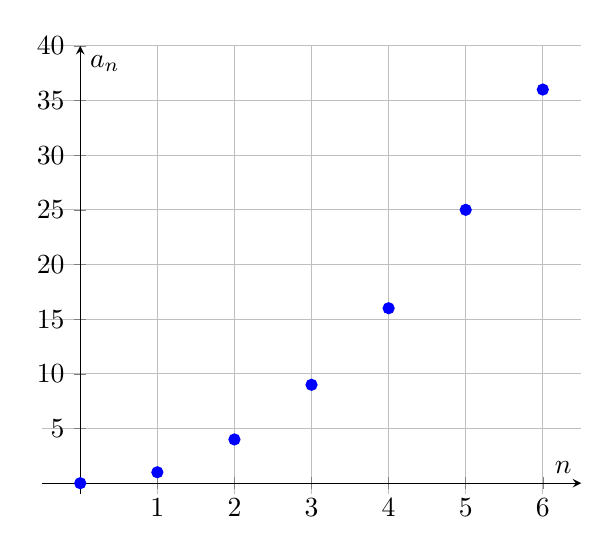
\begin{tikzpicture}
\begin{axis}[
    axis lines = middle,
    xlabel = {$n$},
    ylabel = {$a_n$},
    xmin = -0.5, xmax = 6.5,
    ymin = -1, ymax = 40,
    xtick = {0,1,2,3,4,5,6},
    ytick = {0,5,10,15,20,25,30,35,40},
    grid = both,
]
\addplot[
    only marks,
    mark = *,
    blue
]
coordinates {
    (0,0)
    (1,1)
    (2,4)
    (3,9)
    (4,16)
    (5,25)
    (6,36)
};
\end{axis}
\end{tikzpicture}
\end{center}
\paragraph{Notazione:} di solito invece che con $f(n)$ nelle successioni si indica il termine n-esimo di una successione con $a_n$.\\
Una successione è una sequenza "infinita" di numeri reali $\{a_1, a_2, \ldots\}$.\\
La successione stessa si denota con $\{a_n\}$\\
Esempio di successione:
\[
a_n = \frac{1}{n-5}
\]
\[
S = \{n \in \mathbb{N} : n > 5\}
\]
Esempio di funzione che non è una successione (non esiste una semiretta di numeri naturali per cui la funzione ha senso):
\[
f(n) = \sqrt{5-n} 
\]
\subsection{Limiti di successioni}
L'unico limite che ha senso calcolare per una successione è $n \to +\infty$ perchè $+\infty$ è l'unico punto di accumulazione di una qualsiasi semiretta $\mathbb{N}$.
\[
\lim_{n \to +\infty} a_n = l \in \overline{\mathbb{R}}
\]
Se:
\[
\forall intorno-V-di-l, \exists n_0 : \forall n \geq n_0, a_n \in V
\]
In questo caso si dice che $a_n$ converge a $l$ se $l \in \mathbb{R}$, altrimenti si dice che diverge positivamente o negativamente.\\
Ovviamente, come nelle funzioni normali, il limite può non esistere.\\
\subsection{Sottosuccessioni o successioni "estratte"}
Data $a_n:S \to \mathbb{R}$ come successione, consideriamo una funzione strettamente crescente $K_n:\mathbb{N} \to S$ e consideriamo la composizione $a_{kn}$ una successione, che si definisce \textbf{sottosuccessione} di $\{a_n\}$.\\
\paragraph{Esempio:}
\[
a_n = \frac{1}{n}, S = \{n \in \mathbb{N} : n \geq 1\}
\]
\[
k_n = 2n + 1, \mathbb{N} \to S
\]
\[
b_n = a_{kn} = a_{2n + 1} = \frac{1}{2n + 1}
\]
Un teorema dice:
\[
\lim_{n \to +\infty} a_n = l \Leftrightarrow \lim_{n \to +\infty} a_{kn} = l
\]
\[
\forall k_n(sottosuccessione)
\]
Questo teorema si usa per dimostrare che il limite di una successione \textbf{non esiste}.
\paragraph{Esempio:}
\[
a_n = (-1)^n
\]
Questa funzione ovviamente non ha limite perche se $n$ è pari, il risultato è $1$, se è dispari il risultato sarebbe $-1$.\\
Per dimostrarlo col teorema, prendiamo le due sottosuccessioni $a_{2n}$ e $a_{2n + 1}$.\\
Per assurdo, se $a_n$ convergesse veramente ad $l$, allora anche le sottosuccessioni in questione convergerebbero ad $l$ ed avrebbero quindi lo stesso limite. Questo però è falso e quindi il limite non esiste.\\\\
Per i limiti delle successioni continuano a valere le proprietà viste in precedenza come:
\begin{itemize}
  \item Teorema dei Carabinieri
  \item Permanenza del segno: se $\lim_{n \to +\infty} a_n = l > 0$ allora dopo un certo punto, $a_n$ si terrà sempre sopra 0.
  \item Formule dei limiti come somme, prodotti e quozienti.
\end{itemize}
\subsection{Monotonia di successioni}
Una successione $\{a_n\}$ è:
\begin{itemize}
  \item Debolmente crescente se $n > m \implies a_n \geq a_m$
  \item Strettamente crescente se $n > m \implies a_n > a_m$
  \item Debolmente decrescente se $n > m \implies a_n \leq a_m$
  \item Strettamente decrescente se $n > m \implies a_n < a_m$
\end{itemize}
Inoltre, in particolare, $\{a_n\}$ è:
\begin{itemize}
  \item Debolmente crescente se $a_{n+1} \geq a_n$ $\forall n \in S$
  \item Strettamente crescente se $a_{n+1} > a_n$ $\forall n \in S$
  \item Debolmente decrescente se $a_{n+1} \leq a_n$ $\forall n \in S$
  \item Strettamente decrescente se $a_{n+1} < a_n$ $\forall n \in S$
\end{itemize}
Se una successione è monotona allora ammette limite.\\
Se una successione è crescente allora $l \ne -\infty$ e analogamente se è decrescente allora $l \ne +\infty$.
\subsection{Limitatezza, minimi e massimi}
Una successione $\{a_n\}$ è:
\begin{itemize}
  \item Limitata superiormente se $\exists M \in \mathbb{R} : a_n \leq M$ $\forall n \in S$
  \item Limitata inferiormente se $\exists m \in \mathbb{R} : a_n \geq m$ $\forall n \in S$
  \item Limitata se superiormente e inferiormente limitata.
\end{itemize}
Se una successione è convergente allora è limitata.\\
Se $\lim_{n \to +\infty} a_n = l = +\infty$ allora $a_n$ ha sicuramente un minimo, se invece $l = -\infty$ 
\subsubsection{Teorema di Weierstrass generalizzato per le successioni}
Se $\{a_n\}$ ha limite $l \in \mathbb{R}$ allora:
\begin{itemize}
  \item Ha massimo $\Leftrightarrow \exists n_0 : a_{n_0} \geq l$ 
  \item Ha minimo $\Leftrightarrow \exists n_0 : a_{n_0} \leq l$ 
\end{itemize}
\subsection{Legame tra limiti di funzioni e successioni}
Se abbiamo $A \subseteq \mathbb{R}$, $f:A \to \mathbb{R}$ allora se:
\[
\lim_{x \to x_0} f(x) = l \Leftrightarrow \forall succ\{a_n\} \in A :
\]
\[
\lim_{n \to +\infty} a_n = x_0 
\]
Allora:
\[
\lim_{n \to +\infty} f(a_n) = l
\]
Per dimostrare quindi che una funzione non ha limite basta dimostrare che due successioni associate hanno limite diverso.\\
Di solito come sottosuccessione si prende $\{a_n\} = n$ e quindi $x_0 = +\infty$ e quindi implica che se $\lim_{x \to x_0} f(x) = l$ allora $\lim_{n \to +\infty} f(a_n) = l$.
\paragraph{Esempio:}
\[
\lim_{n \to +\infty} n^2 - 2n = +\infty -\infty = indeterminata
\]
Ponendo $f(x) = x^2 - 2x$, il limite è $+\infty$ (quadrato più veloce)\\\\
Nel caso nella funzione ci sia un $(-1)^n$ bisogna distinguere i casi pari e dispari ($cos(n\pi)$ è equivalente a $(-1)^n$).\\\\
Se abbiamo $\{a_n\}$ come successione con dominio $S \subseteq \mathbb{N}$ e due sottosuccessioni $\{a_{hn}\}$ e $\{a_{kn}\}$ tale che:
\[
\{a_{hn}\} \cup \{a_{kn}\} = S 
\]
Ovvero \textbf{saturano} tutti gli indici, e se esistono i limiti e sono uguali:
\[
\lim_{x \to +\infty} \{a_{hn}\}
\]
\[
\lim_{x \to +\infty} \{a_{kn}\}
\]
Allora $\{a_{n}\}$ ha limite uguale a questi due.
\subsection{Criterio del rapporto}
Il criterio del rapporto si applica quando non si riesce a trovare il limite in altri modi.\\
Se abbiamo una successione $\{a_{n}\}$ \textbf{definitivamente} (da un certo punto in poi) $> 0$ ed esiste il limite dei rapporti:
\[
\lim_{n \to +\infty} \frac{a_n + 1}{a_n} = l \in \overline{\mathbb{R}}
\]
Allora:
\begin{itemize}
  \item Se $0 \leq l < 1$ allora la successione è infinitesima e quindi $\lim_{n \to +\infty} a_n = 0$.
  \item Se $l > 1$ allora $\lim_{n \to +\infty} a_n = +\infty$
  \item Se $l = 1$, non si può concludere niente.
\end{itemize}
Questi criteri funzionano anche per una successione definitivamente negativa, basta cambiare il segno del limite.\\
\paragraph{Esempio:}
\[
\lim_{n \to +\infty} \frac{1}{2}^n
\]
Questo si potrebbe risolvere anche senza criterio del rapporto facendolo diventare $\frac{1}{2^n}$, ma proviamo comunque:
\[
\lim_{n \to +\infty} \frac{a_{n+1}}{a_n} = \frac{\frac{1}{2}^{n+1}}{\frac{1}{2}^n} = \frac{1}{2} < 1
\]
Quindi il limite è $0$.
\paragraph{Gerarchia di crescita:} $n^n >> n! >> b^n >> n^k$
\subsection{Criterio della radice}
Se abbiamo una successione $\{a_{n}\}$ \textbf{definitivamente} $> 0$ ed esiste il limite:
\[
\lim_{n \to +\infty} \sqrt[n]{a_n} = l \in \overline{\mathbb{R}}
\]
Allora:
\begin{itemize}
  \item Se $0 \leq l < 1$ allora la successione è infinitesima e quindi $\lim_{n \to +\infty} a_n = 0$.
  \item Se $l > 1$ allora $\lim_{n \to +\infty} a_n = +\infty$
  \item Se $l = 1$, non si può concludere niente.
\end{itemize}
\paragraph{Dimostrazione punto 1:} supponiamo $\sqrt[n]{a_n} = l$ e che $0 \leq l < 1$, scegliamo $m \in \mathbb{R} : l < m < 1$.\\
Ad esempio $m = \frac{l + 1}{2}$ (sicuramente tra $l$ e 1).
Dato che $l < m$ allora definitivamente:
\[
\sqrt[n]{a_n} < m \implies a_n < m^n
\]
$m^n = 0$ perche $m < 1$ e quindi $a_n < 0$, tende a 0.
\paragraph{Dimostrazione punto 2:} stavolta $m \in \mathbb{R} : 1 < m < l$ e segue che definitivamente $\sqrt[n]{a_n} > m$, $a_n > m^n$, quindi $m^n$ tende a $+\infty$ e quindi anche $\{a_n\}$\\\\
Secondo un teorema, se esiste il limite dei rapporti allora esiste anche il limite del criterio della radice e sono uguali, ma non è sempre vero il contrario e il teorema vale anche per $l = 1$.
\paragraph{Curiosità:} $\sqrt[n]{P(n)} = 1$, dato questo se $a_n$ è compreso tra due polinomi allora il limite sarà $1$ per via del teorema dei Carabinieri.

\section{Serie numeriche}
Sia $\{a_n\}$ una successione, si definisce la \textbf{somma parziale} ennesima come:
\[
S_n = \sum_{j=0}^{n} a_j = a_0 + a_1 + \cdots + a_n
\]
La \textbf{serie} associata alla successione è il limite di tale $S_n$ se $n \to \infty$.\\
\[
\sum_{j=0}^{+\infty} a_j = \lim_{n \to +\infty} S_n
\]
Potremmo pensare che una somma di infiniti termini positivi sia sempre $= +\infty$, ma non è sempre così, vediamo un esempio:\\
\[
a_n = \frac{1}{2^n}, n > 1
\]
\[
S_n = \frac{1}{2} + \frac{1}{4} + \frac{1}{8} + \cdots
\]
Geometricamente, ogni volta si passa al punto medio del segmento rimanente per arrivare a $1$, per esempio quando si aggiunge $\frac{1}{2}$ manca $\frac{1}{2}$ per arrivare a 1, ma si aggiunge $\frac{1}{4}$, e così via.\\
Non si arriva mai ad 1, ma ci si avvicina sempre di più, quindi la serie è $1$.\\
Ovviamente una serie, essendo un limite, può non esistere, in tal caso si dice che non esiste o che è indeterminata.\\
Se esiste, può convergere, diverge positivamente o negativamente.\\\\
Il valore di una serie o il suo comportamento è identico a quello della serie realizzata con la somma dei termini della stessa successione partendo dal k-esimo termine. Si dice che una serie ha lo stesso comportamento di una sua qualsiasi coda.
\subsection{Serie notevoli}
\paragraph{Serie geometrica:}
\[
\alpha \in \mathbb{R}, a_n = \alpha^n
\]
\[
S_n = \alpha^0 + \alpha^1 + \cdots = \frac{\alpha^{n+1} - 1}{\alpha - 1}
\]
La serie può essere:
\begin{itemize}
  \item $+\infty$ se $\alpha \geq 1$
  \item $\frac{1}{1 - \alpha}$ se $|\alpha| < 1$
  \item inesistente se $a \leq -1$
\end{itemize}

\paragraph{Inverso del fattoriale:}
\[
a_n = \frac{1}{n!}
\]
\[
S_n = 1 + 1 + \frac{1}{2} + \frac{1}{6} + \cdots = e
\]
Questo si può dimostrare con la formula di Taylor con resto di Lagrange.

\subsection{Teorema di condizione necessaria per la convergenza di una serie}
Se $\{a_n\}$ è una successione e la sua serie $\sum_{n=0}^{+\infty} a_n$ converge, allora la $a_n$ è infinitesima, ovvero tende a $0$ per $n \to +\infty$\\
Lo abbiamo gia visto nel primo esempio, andiamo a sommare qualcosa di sempre più piccolo.\\
Con quest si può dire che se $\{a_n\}$ non è infinitesima, allora la serie diverge (non si può concludere se positivamente o negativamente).\\\\
Attenzione: non è vero che se $\{a_n\} \to 0$ allora la serie converge, ma solo il contrario.

\subsection{Teorema della somma e prodotto per le serie}
Se $\{a_n\}$ e $\{b_n\}$ sono successioni e $\sum_{n=0}^{+\infty} a_n$ e $\sum_{n=0}^{+\infty} b_n$ esistono, allora:
\[
\sum_{n=0}^{+\infty} (a_n + b_n) = \sum_{n=0}^{+\infty} a_n + \sum_{n=0}^{+\infty} b_n
\]
A meno che la serie risultante sia indeterminata, in tal caso si somma semplicemente $a_n + b_n$ e si trova un $c_n$ per poi svolgere la serie su di esso.\\
Alternativamente, si può ricorrere al confronto asintotico o gerarchia di infiniti.\\\\
NON vale:
\[
\sum_{n=0}^{+\infty} (a_n \cdot b_n) = \sum_{n=0}^{+\infty} a_n \cdot \sum_{n=0}^{+\infty} b_n
\]
Si creerebbero monomi misti e non avrebbe senso.
\subsection{Serie definitivamente a termini positivi}
Consideriamo $\sum_{n=0}^{+\infty} a_n$ in cui $a_n > 0$ definitivamente (dopo un certo punto).\\
Dato che come già affermato ogni serie si comporta nello stesso modo di ogni sua coda, basta lavorare sulla coda che parte dal punto in cui $a_n > 0$ definitivamente.\\
Se $a_n \geq 0$ definitivamente allora $\sum_{n=0}^{+\infty} a_n$ converge o diverge a $+\infty$, altrimenti ($a_n \leq 0$ definitivamente), può convergere o divergere a $-\infty$
\subsection{Teorema del confronto}
Se $\{a_n\}$ e $\{b_n\}$ sono successioni e definitivamente:
\[
0 \leq a_n \leq b_n
\]
Allora:
\begin{itemize}
  \item Se $\sum_{n=0}^{+\infty} b_n$ converge, allora anche $\sum_{n=0}^{+\infty} a_n$ converge.
  \item Se $\sum_{n=0}^{+\infty} a_n$ diverge, allora anche $\sum_{n=0}^{+\infty} b_n$ diverge.
\end{itemize}
La definizione è analoga se $b_n \leq a_n \leq 0$, basta lavorare sui valori opposti e ottenere il valore opposto della serie, dato che in fondo si tratta di una semplice somma.
\subsection{Teorema del confronto asintotico}
Se abbiamo $\{a_n\}$ e $\{b_n\}$ come successioni definitivamente positive e se:\
\[
\lim_{n \to + infty} \frac{a_n}{b_n} = l \in \overline{\mathbb{R}}  
\]
Allora se:
\begin{itemize}
  \item $l \in (0,+\infty) \implies \sum_{n=0}^{+\infty} b_n$ e $\sum_{n=0}^{+\infty} a_n$ hanno lo stesso comportamento.
  \item $l = 0 \implies $ se $\sum_{n=0}^{+\infty} b_n$ converge, allora anche $\sum_{n=0}^{+\infty} a_n$ converge.
  \item $l = +\infty \implies$ se $\sum_{n=0}^{+\infty} b_n$ diverge, anche $\sum_{n=0}^{+\infty} a_n$ diverge.
\end{itemize}
\subsection{Criterio della radice per le serie}
Si ha una successione $\{a_n\}$ definitivamente positiva, se esiste:
\[
\lim_{n \to \infty} \sqrt[4]{a_n} = l \in \overline{\mathbb{R}}
\]
Allora:
\begin{itemize}
  \item $0 \leq l < 1 \implies \sum_{n=0}^{+\infty} a_n$ converge
  \item $l > 1 \implies \sum_{n=0}^{+\infty} a_n$ diverge. 
  \item $l = 1 \implies$ niente, non si conclude niente.
\end{itemize}
\subsection{Criterio del rapporto per le serie}
Si ha una successione $\{a_n\}$ definitivamente positiva, se esiste:
\[
\lim_{n \to \infty} \frac{a_{n+1}}{a_n} = l \in \overline{\mathbb{R}}
\]
Allora:
\begin{itemize}
  \item $0 \leq l < 1 \implies \sum_{n=0}^{+\infty} a_n$ converge
  \item $l > 1 \implies \sum_{n=0}^{+\infty} a_n$ diverge. 
  \item $l = 1 \implies$ niente, non si conclude niente.
\end{itemize}
Questo criterio si può applicare anche a successioni definitivamente negative, basta operare sul loro opposto ($-a_n$).
\subsection{Legame con integrali impropri}
Una serie può essere vista come un integrale improprio:
\[
f:(0,+\infty) \to \mathbb{R}
\]
\[
f(x) = [x]
\]
\[
\sum_{n=0}^{+\infty} a_n = \int_{0}^{+\infty} f(x)
\]
\subsection{Criterio dell'integrale}
$\overline{n} \in \mathbb{N}$, $f:(\overline{n},+\infty) \to \mathbb{R}$ debolmente crescente, $f(x) \geq 0$ sempre, $a_n = f(n)$ allora $\sum_{n=0}^{+\infty} a_n$ e $\int_{\overline{n}}^{+\infty} f(x)dx$ si comportano nello stesso modo.
\subsection{Criterio dell'assoluta convergenza}
$\{a_n\}$ è una successione.
\paragraph{Convergenza assoluta:} $\{a_n\}$ converge assolutamente se $\sum_{n=0}^{+\infty} |a_n|$ converge.
Se $\sum_{n=0}^{+\infty} a_n$ converge assolutamente allora converge e $|\sum_{n=0}^{+\infty} a_n| = \sum_{n=0}^{+\infty} |a_n|$
\subsection{Serie a segno alterno}
Sia $\{a_n\}$ una successione, è a segno alterno se è nella forma:
\[
\sum_{n=0}^{+\infty} (-1)^n \cdot a_n
\]
Dove $a_n$ è una successione con segno costante.
\subsection{Criterio di Leibnitz}
$\{a_n\}$ è una successione definitivamente $\geq 0$, debolmente crescente.\\
Se $\lim_{n \to +\infty} a_n = 0$ allora $\sum_{n=0}^{+\infty} (-1)^n \cdot a_n$ converge a $0$.

\section{Analisi a più variabili}
Di solito si lavora con due variabili, ma spesso le definizioni si basano su un numero generico di variabili.\\
Fino ad ora le funzioni erano nella forma $f:A \to \mathbb{R}$, adesso sono nella forma:
\[
f:\Omega \to \mathbb{R}^n
\]
Con:
\[
\Omega \subset \mathbb{R}^n
\]
\paragraph{Geometricamente:}
\begin{itemize}
  \item $n = 1 \implies \mathbb{R}$, una dimensione.
  \item $n = 2 \implies \mathbb{R}^2$, un piano bidimensionale.
  \item $n = 3 \implies \mathbb{R}^3$, uno spazio tridimensionale.
  \item $n > 3 \implies $ non si può immaginare ma è uno spazio valido.
\end{itemize}
In generale, $\mathbb{R}^n$ è uno \textbf{spazio vettoriale} in cui vale la somma:
\[
(x_1,\ldots,x_n) + (y_1,\ldots,y_n) = (x_1 + y_1, \ldots, x_n + y_n)
\]
e la moltiplicazione per scalare:
\[
\lambda \cdot (x_1,\ldots,x_n) = (\lambda \cdot x_1,\ldots, \lambda \cdot x_n)
\]
$\mathbb{R}^2$ e $\mathbb{R}^3$ si possono vedere come la somma e il prodotto per scalare dei \textbf{vettori geometrici} corrispondenti ($x,y,z$) (concetto di \textbf{base} in algebra)
\subsection{Norme e distanze}
Se $x = (x,\ldots,x_n) \in \mathbb{R}^n$, la sua \textbf{norma} è:
\[
||x|| = \sqrt{x \cdot x} = \sqrt{x_1^2 + x_2^2 + \cdots + x_n^2}
\]
Una \textbf{distanza} tra due elementi $x = (x_1,\ldots,x_n), y = (y_1,\ldots,y_n)$ è:
\[
d(x,y) = ||x-y|| =\sqrt{(x_1 - y_1)^2 + \cdots + (x_n - y_n)^2}
\]
La distanza tra due punti su un piano infatti è proprio questa.\\\\

\subsection{L'angolo tra vettori}
Il prodotto scalare $<x,y>$ è collegato all'angolo formato dai due vettori:
\[
<x,y> = ||x|| \cdot ||y|| \cdot cos(\theta)
\]
\[
\theta = \arccos(\frac{<x,y>}{||x|| \cdot ||y||})
\]
$\theta$ è:
\begin{itemize}
  \item Acuto $(0 < \theta < \frac{\pi}{2})$ se $<x,y> > 0$
  \item Ottuso $(\frac{\pi}{2} < \theta < \pi)$ se $<x,y> < 0$
  \item Retto $(\theta = \frac{\pi}{2})$ se $<x,y> = 0$
\end{itemize}
\paragraph{Esempio:} troviamo l'angolo tra i vettori $(1,1,1)$ e $(1,1,0) \in \mathbb{R}^3$
\[
||(1,1,0)|| = \sqrt{1+1+0} = \sqrt{2}
\]
\[
||(1,1,1)|| = \sqrt{1+1+1} = \sqrt{3}
\]
\[
<x,y> = (1,1,0) \cdot (1,1,1) = 1+1+(0 \cdot 1) = 2
\]
\[
\theta = \frac{2}{\sqrt{2} \cdot \sqrt{3}}
\]
\[
\theta = \frac{2}{\sqrt{6}}
\]
\[
\theta = \frac{2\cdot \sqrt{6}}{6}
\]
\[
\theta = \frac{\sqrt{6}}{3}
\]
\[
\theta = \arccos(\frac{\sqrt{6}}{3})
\]

\subsection{Sottoinsiemi importanti dell'insieme dei Reali alla n}
Dati:
\[
x \in \mathbb{R}^n, r \in \mathbb{R} \geq 0
\]
Definiamo alcuni sottoinsiemi di $\mathbb{R}^n$:\\
La \textbf{palla aperta} centrata in $x$ e di raggio $r$ è:
\[
B(x,r) = B_r(x) = \{y \in \mathbb{R}^n : d(x,y) < r\}
\] 
Ovvero tutti i punti distanti al massimo quanto il raggio da $x$.\\
Per:
\begin{itemize}
  \item $n = 1:$ intervallo con punto medio uguale a $x$ con estremi $(x-r,x+r)$
  \item $n = 2:$ disco / cerchio su un piano
  \item $n = 3$ sfera
\end{itemize}
Una \textbf{palla chiusa} è la stessa cosa ma include gli estremi, ovvero $d(x,y) \leq r$.\\
La palla che invece include SOLTANTO gli estremi ha $n-1$ dimensioni, infatti per:
\begin{itemize}
  \item $n = 1:$ 0 dimensioni in quanto contiene solo due punti distinti.
  \item $n = 2:$ solo la circonferenza, 1 dimensione
  \item $n = 3:$ solo il bordo della sfera
\end{itemize}
Se $E \subseteq \mathbb{R}^n$, definiamo il \textbf{complementare} di E:
\[
E^c = \mathbb{R}^n \setminus E
\]
\subsection{Punti interni, esterni e di bordo}
$x_0 \in \mathbb{R}^n$ è definito \textbf{punto interno} di $E$ se $x_0 \in E$ e $\exists r > 0 : B(x,r) \subseteq E$, ovvero se esiste una palla che sta completamente dentro $E$.\\
La definizione di \textbf{punto esterno} è analoga: $x_0 \notin E$ e $\exists B(x,r) \subseteq E^c$.\\
Un \textbf{punto di bordo o di frontiera} è un punto che non è ne' interno ne' esterno, ovvero non importa quanto piccolo $r$ sia, qualsiasi palla centrata in $x_0$ avrà sia elementi di $E$ che di $E^c$.\\
La \textbf{parte interna} di $E$ è l'unione di tutti i suoi punti interni e si indica con $E$ con una $o$ sopra (non avevo il simbolo).\\
Il \textbf{bordo o frontiera} di $E$ è l'unione di tutti i suoi punti di bordo e si indica con $\partial E$.\\
Se $x \in \mathbb{R}^n$ e $E \subseteq \mathbb{R}^n$, $x$ è un \textbf{punto di accumulazione} di $E$ se $\forall r > 0$:
\[
B(x,r) \setminus {x} \cap E \ne \emptyset
\]
Ovvero una palla centrata in tale punto interseca $E$ almeno in un punto che non sia il centro.\\
Se questo non accade, $x$ è un \textbf{punto isolato}.\\
/subsection{Proprietà sottoinsiemi}
Un \textbf{sottoinsieme aperto} è costituito solo da punti interni ($\partial E \cap E = \emptyset$), mentre un \textbf{sottoinsieme chiuso} comprende anche punti di bordo (($\partial E \subseteq E$)).\\
Esistono sottoinsiemi ne' aperti ne' chiusi, come $[0,1]$ escluso $1$ (non potevo usare la parentesi tonda), perche le due condizioni appena riportate non sono verificate.\\
L'intersezione di due sottoinsiemi aperti è aperto.\\
L'unione di più sottoinsiemi aperti è aperto.
\subsection{Insiemi limitati e R alla n esteso}
Un \textbf{insieme limitato} è un sottoinsieme $E \subseteq \mathbb{R}^n$ che è contenuto in una palla qualsiasi.\\
Questo equivale a dire che esso deve essere contenuto in una palla con centro origine e raggio qualsiasi perchè ogni palla esistente è contenuta in una palla con centro origine.\\
Se $E$ quindi è contenuto in tale palla allora:
\[
\exists r \in \mathbb{R} > 0 : E \subseteq B(0,r)
\]
e quindi:
\[
\forall x \in E \implies d(x,0) < r
\]
Ovvero ogni punto è meno distante del raggio dall'origine.\\
Vediamo adesso alcuni dettagli:
\begin{itemize}
  \item Tutte le palle sono limitate
  \item $\mathbb{R}^n$ non è limitato
  \item una retta o un piano in $\mathbb{R}^3$ non sono limitati in quanto si estendono all'infinito.
\end{itemize}
Adesso estendiamo $\mathbb{R}^n$ aggiungendo un \textbf{punto all'infinito}.\\
In $\mathbb{R}$ ricordiamo che bastava aggiungere $+\infty$ e $-\infty$.\\
In $\mathbb{R}^2$ ci si può allontanare in molti più modi all'infinito dall'origine, per semplicità quindi si aggiunge solo un punto a cui ci si avvicina allontanandosi all'infinito in qualsiasi modo.\\
Definiamo:
\[
\overline{\mathbb{R}^n} = \mathbb{R}^n \cup \{\infty\}
\]
Un intorno di $\infty$ è il complementare della palla $B(0,a)$ per un $a$ abbastanza grande.\\
Il punto all'infinito è un punto di accumulazione di $E$ se $E$ è non limitato.
\subsection{Descrizione esplicita di sottoinsiemi in R alla n}
Per $\mathbb{R}^2$, una retta è determinata da due punti qualsiasi $P,Q$ diversi.\\
Il \textbf{vettor differenza} ($Q - P$) è il \textbf{vettore direzione} della retta.\\
Ogni punto della retta si trova sommando a $P$ un multiplo qualsiasi di $(Q-P)$.\\
In formula, $\binom{x}{y} \in \mathbb{R}^2$ sta sulla retta data se:
\[
\exists t : \binom{x}{y} = P + t(Q-P)
\]
Ovvero:
\[
\begin{cases}
  x = x_1 + t(x_2 - x_1)\\
  y = y_1 + t(y_2 - y_1)
\end{cases}
\]
Con $Q = 2$ e $P = 1$.\\
Sappiamo che $ax + by + c$ è la formula della retta generica, con questo diciamo che il vettore $(a,b)$ è ortogonale a $(Q,P)$.\\
Per trovare un vettore da un dato $(a,b)$ bisogna trovare un vettore che annulli l'equazione $(a,b)(Q,P) = 0$, ovvero $(-b,a)$. Per esempio troviamo la retta per $(1,2)$ e $(3,5)$:
\[
\begin{cases}
  x = 1 + t(3 - 1) \\
  y = 2 + t(5 - 2)
\end{cases}
\]
E si svolge per un qualsiasi $t$.\\
Un'equazione di una retta non è unica infatti.\\
Tutto questo è analogo per $n=3$, ma con parametri in più.\\
Anche i piani si possono rappresentare in forma parametrica come una \textbf{base}:
\[
\lambda(Q - P) + \mu(Q_2 - P)
\]
\subsection{Curve nel piano e nello spazio tridimensionale}
Una \textbf{curva} in $\mathbb{R}^2$ è una funzione:
\[
\gamma : I \to \mathbb{R}^2
\]
Dove $I \subseteq \mathbb{R}$ è un intervallo.\\
Al variare di $t \in I$ (che si pensa come il "tempo") il punto $\gamma(t)$ descrive una curva.\\
Una funzione $\gamma: I \to \mathbb{R}^2$ è determinata da due funzioni:
\begin{itemize}
  \item $x(t): I \to \mathbb{R}$
  \item $y(t): I \to \mathbb{R}$
\end{itemize}
E quindi:
\[
\gamma(t) = \gamma(x(t),y(t))
\]
Il \textbf{sostegno} di una curva è l'immagine di $\gamma$ come sottoinsieme di $\mathbb{R}^2$.
\paragraph{Esempio:} $\gamma(t) = (cost(t),sin(t)), I = [0, 2\pi]$\\
$\gamma$ è una curva il cui sostegno è esattamente la circonferenza unitaria (centro 0, raggio 1), percorsa 1 volta in senso antiorario.\\
Se $I = [0,6\pi]$ la curva avrà lo stesso sostegno ma percorre la circonferenza tre volte.\\
Intuitivamente, esistono infinite curve per un solo sostegno.\\
Inoltre, ogni grafico di ogni funzione in 1 variabile è un sostegno di una curva di $\mathbb{R}^2$:
\[
f: I \to \mathbb{R} \implies \gamma(t) = (t,f(t))
\]
Quando una curva torna su se stessa si dice che è \textbf{chiusa} se i due estremi sono uguali (e quindi $I$ è della forma $[a,b]$) e \textbf{semplice} se non torna mai su se stessa ad esclusione degli estremi, ovvero $\gamma$ è iniettiva all'interno dell'intervallo $I$.\\
Tutto questo è analogo per $\mathbb{R}^3$.
\[
\gamma(t) = (x(t),y(t),z(t))
\]
\paragraph{Osservazione:} per dire che un $\gamma$ è semplice o meno, basta che tra le funzioni delle coordinate ci sia almeno una funzione iniettiva, se non c'è potrebbe essere non semplice.\\\\
Data una curva, il suo \textbf{vettore tangente} in $\gamma(t_0) = (x(t_0),y(t_0))$ è (gamma qui dovrebbe avere un pallino pieno sopra se stesso (il simbolo)):
\[
\gamma(t_o) = (x^|(t_0),y^|(t_0))
\]
Se questo esiste, la \textbf{retta tangente} a $\gamma$ per $t \to t_0$ è $\gamma(t_0)$ (con pallino).
\subsection{Funzioni a più variabili}
Una funzione in $\mathbb{R}^n$ è una tripla ($\Omega,B,f$), dove:
\begin{itemize}
  \item $\Omega \subseteq \mathbb{R}^n$ è il dominio
  \item $B \subseteq \mathbb{R}$ è il codominio
  \item $f$ è una "regola" (formula) che associa elementi del dominio a elementi del codominio.
\end{itemize}
Proprio come una funzione classica!\\
Il \textbf{grafico} di tale funzione è:
\[
Graph(f) = \{(x_1,\ldots,x_n,x_{n+1}) : x_{n+1} = f(x_1,\ldots,x_n)\}
\]
Un \textbf{insieme di livello} $\lambda$ (tipicamente una curva) di una funzione è l'insieme di tutti i punti ad un certo livello.\\
Per esempio, tutti i punti della funzione con $z = 5$.
\subsection{Limiti di funzioni con più variabili}
Il \textbf{limite} di una funzione con più variabili (vediamo 2 variabili) per ($x,y$) che tende a ($x_0,y_0$) è uguale a $l \in \overline{R}$ e si scrive:
\[
\lim_{(x,y) \to (x_0,y_0)} f(x,y) = l
\]
Se $\forall$ intorno di $l$ esiste un intorno $U$ di $(x_0,y_0) : (x,y) \in U \setminus \{x_0,y_0\} \implies f(x,y) \in V$.\\
La definizione è praticamente la stessa dei limiti normali, ma adesso l'intorno è una palla aperta.\\
Se $l \in \mathbb{R}$, la palla è $U = B_{\delta}(x_0,y_0)$\\
Una funzione $f:\Omega \to \mathbb{R}$ è \textbf{continua} in $(x_0,y_0) \in \Omega$ se $\lim_{(x,y) \to (x_0,y_0)} f(x,y)$ esiste ed è uguale a $f(x_0,y_0)$.
Tutti gli strumenti e teoremi affrontati nell'analisi dei limiti per funzioni ad una variabile valgono anche per le funzioni a più variabili, come il teorema dei carabinieri, del confronto, della permanenza del segno...\\
\paragraph{Esempio di calcolo:} $\lim_{(x,y) \to (x_0,y_0)} \frac{xy}{x^2 + y^2}$\\
Forma indeterminata, dominio $= \mathbb{R}^2 \setminus \{(0,0)\}$. Prima di tutto si prova a restringere la funzione a una retta passante per $(0,0)$ e calcolare il limite lungo quella retta.\\
Per esempio, se $y = 0$ sempre allora è vincolata a stare sull'asse delle $x$. Il limite in questo caso fa $0$.\\
Proviamo anche il contrario, ovvero con $x = 0$, il limite vale di nuovo $0$.\\
Proviamo adesso con la bisettrice $y = x$, che in forma di curva è $(t,t)$:
\[
f((t,t)) = \frac{t^2}{t^2 + t^2} = \frac{t^2}{2t^2} = \frac{1}{2} 
\]
Questo è un limite diverso da quelli di prima, quindi il limite generale non esiste.\\\\
Formalmente, il limite di una funzione a più variabili esiste se è uguale per tutti i modi in cui mi avvicino.\\
Infatti, secondo un teorema, se il limite esiste allora per ogni curva che interseca ($x_0,y_0$) il limite è lo stesso (si usa per dimostrare la non esistenza).
Purtroppo per concludere che il limite esiste non basta provare che ogni curva ha lo stesso limite.
\subsubsection{Coordinate polari}
Se ogni metodo per calcolare un limite fallisce (carabinieri e altro) allora si possono usare le \textbf{coordinate polari} ($\rho,\theta$):
\begin{itemize}
  \item $\rho = $ distanza dal centro del punto
  \item $\theta = $ angolo che forma il punto con l'asse $x$ ($\theta \in [0,2\pi]$ con estremo superiore escluso)
\end{itemize}
Nell'origine $\theta$ non è definito, si indica con $\rho = 0$.\\
Vediamo le formule di conversione ($\theta$ ci interessa poco):
\[
\begin{cases}
  x = \rho cos(\theta)\\
  y = \rho sin(\theta)\\
  \rho = \sqrt{x^2 + y^2}\\
  \theta = arcos(\frac{x}{\sqrt{x^2,y^2}}), y > 0\\
  \theta = 2\pi - arcos(\frac{x}{\sqrt{x^2,y^2}}), y < 0
\end{cases}
\]
Le coordinate polari sono utili per i limiti che tendono all'origine perche significa che $\rho \to 0$.\\
Per risolvere esercizi, si sostituiscono i valori con le coordinate polari, se il risultato dipende da $\theta$ allora il limite non esiste, altrimenti esiste:
\[
\rho \to +\infty, \theta limitato, \rho \cdot \theta \implies \text{ limite esiste perche theta è limitato}
\]

\subsection{Derivate in più variabili}
\subsubsection{Derivate parziali}
La derivata in più variabili si può trovare definendo prima le \textbf{derivate parziali}, derivando solo ad una variabile, lasciando le altre "fissate" (si trattano come costanti, ma senza attribuirgli uno specifico valore).\\
\begin{tikzpicture}
\draw[->] (-1,0) -- (5,0) node[right] {$x$};
\draw[->] (0,-1) -- (0,5) node[above] {$y$};

% horizontal line y = y_0
\draw[blue] (-1,2) -- (5,2) node[right] {$y = y_0$};

% point (x_0, y_0)
\filldraw[red] (3,2) circle (2pt) node[above right] {$(x_0, y_0)$};
\end{tikzpicture}
Si vincola $y$ a $y_0$ e si fa la derivata con solo $x$ ($n=2$).\\
Faccio muovere $(x,y)$ sulla retta $y = y_0$ e guardo la "\textbf{variazione istantanea} di $f(x,y_0)$ nel punto $x = x_0$.\\\\
Una funzione $f:\Omega \to \mathbb{R}$, con $(x_0,y_0) \in \Omega \subseteq \mathbb{R}^2$, si dice che $f$ è \textbf{derivabile parzialmente} rispetto a $x$ in $(x_0,y_0)$ se esiste il limite:
\[
\lim_{h \to 0} \frac{f(x_0 + h, y_0) - f(x_0,y_0)}{h}
\]
Questo, se esiste, è la \textbf{derivata parziale} di $f$ rispetto a $x$ nel punto $(x_0,y_0)$, si indica cosi:
\[
\frac{\delta f}{\delta x} (x_0,y_0)
\]
\[
f_x(x_0,y_0)
\]
\[
D_x f(x_0,y_0)
\]
Il simbolo nella prima denotazione è sbagliato ma non c'erano alternative in latex (è simile ma con ciuffo a sinistra).\\
La definizione è analoga per ogni altra variabile.\\
Queste sono definite le \textbf{derivate solite} di una funzione:
\[
g(h) = f(x_0 + h, y_0)
\]
\[
\lim_{h \to 0} \frac{f(x_0 + h, y_0) - f(x_0,y_0)}{h} = \lim_{h \to 0} \frac{g(h) - g(0)}{h} = g^|(h)
\]
In generale quindi, se $f:\Omega \to \mathbb{R}$ è una funzione e $x_0 \in \Omega \subseteq \mathbb{R}^n$, e quindi $x_0 = (x_1,\ldots,x_n)$, la derivata parziale di $f$ rispetto a $x_k$ nel punto $x_0$ è, se esiste:
\[
\lim_{h \to 0} \frac{f(x_0 + be_k, y_0) - f(x_0)}{h}
\]
Con $e_k = (0,\ldots,1,\ldots,0)$, muovo solo la variabile $k$.\\\\
Ciascuna derivata parziale è a sua volta una funzione.\\\\
Per calcolare le derivate parziali, si usano le solite regole per le derivate in 1 variabile facendo finta che le variabili che non stiamo derivando siamo delle costanti (ma senza un valore attribuito).
\paragraph{Esempio:}
\[
f(x,y) = x^3 + 3xy + y^7
\]
Deriviamo per x, y diventa costante.
\[
\frac{\delta f}{\delta x} = 3x^2 + 3y + 0 = 3x^2 + 3y
\]
\subsubsection{Derivate direzionali}
Per trovare una \textbf{derivata direzionale} si ripete quello che abbiamo fatto per $\frac{\delta f}{\delta x}$, ma con direzione arbitraria invece che $(1,0)$.\\
Fisso $(x_0,y_0) \in \Omega$, $f:\Omega \to \mathbb{R}$ e un \textbf{vettore direzione} $v \ne 0$. Consideriamo la variazione istantanea della $f$ in $(x_0,y_0)$ in direzione $v$ il limite:
\[
\lim_{h \to 0} \frac{f((x_0, y_0) + hV) - f(x_0,y_0)}{h}
\]
\[
h = (\alpha,\beta,\ldots)
\]
Si effettua un prodotto scalare:
\[
\lim_{h \to 0} \frac{f(x_0 \cdot \alpha, y_0 \cdot \beta) - f(x_0,y_0)}{h}
\]
Geometricamente, ci si muove lungo un vettore.\\
Se tale limite esiste, è la derivata direzionale di $f$ per una direzione $v$ ed è $\frac{\delta f}{\delta v}(x_0,y_0)$.\\
Muoversi sull-asse $x$ o $y$ è come avere $\alpha = 0$ o $\beta = 0$.\\
Anche queste sono derivate di una funzione ad 1 variabile se:
\[
g(h) = f(x_0 + h\alpha, y_0 + h\beta)
\]
Per $n \geq 3$, la derivata direzionale di $f$ in $x_0$ in direzione $V$ è:
\[
\lim_{h \to 0} \frac{f(x_0 \cdot hV) - f(x_0)}{h}
\]
Con $x_0 \in \mathbb{R}^n$
\subsubsection{Gradiente}
Se $f:\mathbb{R}^n \to \mathbb{R}$ ammette tutte le derivate parziali in un punto $x_0$, si definisce il \textbf{gradiente} di $f$ in $x_0$ con:
\[
\nabla f(x_0) = (\frac{\delta f}{\delta x} (x_0),\ldots,\frac{\delta f}{\delta x_n} (x_0))
\]
A volte questo è definito come "derivata totale di $f$ in $x_0$" ($x_0 \in \mathbb{R}^n$)
\subsubsection{Differenziabilità}
Se $f: \mathbb{R}^2 \to \mathbb{R}$, $f$ si dice \textbf{differenziabile} in $(x_0,y_0)$ se:
\[
\exists \alpha,\beta \in \mathbb{R} : f(x_0 + h, y_0 + k) = f(x_0,y_0) + (\alpha \cdot h) + (\beta \cdot k) + o(||(h,k)||)
\]
Come si può vedere, c'è un errore di lunghezza del vettore.\\
Se $f$ è differenziabile, esistono tutte le derivate parziali, ma non è vero il contrario.\\
La condizione analoga per $f:\mathbb{R}^n \to \mathbb{R}$ è:
\[
\exists \alpha,\beta \in \mathbb{R}^n : f(x_0 + v) = f(x_0) + \alpha \cdot v
\]
Se $f$ è differenziabile allora:
\begin{enumerate}
  \item $f$ è continua in $x_0$
  \item Esistono tutte le derivate direzionali e quindi anche il gradiente
  \item $\forall v \in \mathbb{R}^n \setminus \{0\}$, $\frac{\delta f}{\delta v}(x_0) = \nabla f(x_0) \cdot v$ (ovvero esiste il gradiente)
  \item l'$\alpha \in \mathbb{R}^n$ nella definizione di differenziale è a posteriori uguale a $\nabla f(x_0) \cdot v$, ovvero:
  \[
  f(x_0,v) = f(x_0) + \nabla f(x_0) \cdot v + o(||v||)
  \]
\end{enumerate}
\paragraph{Dimostrazione punto 2 e 3:}
Calcoliamo:
\[
\frac{\delta f}{\delta w}(x_0)
\]
\[
v \in \mathbb{R}^n
\]
\[
w \ne 0 \text{ fissato}
\]
\[
\frac{\delta f}{\delta w}(x_0) = \lim_{t \to 0} \frac{f(x_0 + tw) - f(x_0)}{t} = \ldots
\]
(Definizione di Differenziabilità con $v = tw$)
\[
\ldots = \lim_{t \to 0} \frac{f(x_0) + \alpha \cdot (tw) + o(||tw||) - f(x_0)}{t}  = \ldots
\]
\[
\ldots = \lim_{t \to 0} \frac{(tw) \cdot \alpha}{t} = \lim_{t \to 0} w \cdot \alpha
\]
\[
\frac{\delta f}{\delta w}(x_0) = w \cdot \alpha
\]
Questa uguaglianza vale sempre.\\
Se $w = e_k$ della forma $(0, \ldots, 1, \ldots, 0)$ ("1" nel posto $k$) allora troviamo:
\[
\frac{\delta f}{\delta w}(x_k) = \frac{\delta f}{\delta e_k}(x_0) = e_k \cdot \alpha = \alpha_k
\]
Si vede proprio che la derivata direzionale per $e_k$ è proprio la derivata parziale con $x_k$.\\
Segue che $\alpha$ è il gradiente di $f$.\\
\subsection{Geometria del vettore gradiente}

\end{document}
